
\section{Experiment}
\label{ch:experiment}

\epigraph{That men do not learn very much from the lessons of history is the most important of all the lessons that history has to teach.}{Aldous Huxley}

\subsection{User Study Process}

\subsection{likert Scale}
The statistics of the questionnaire about system evaluation by using likert scale are shown in figure \ref{figure:1}.

\begin{figure}[h]
\caption{Feedback question about system evaluation}
\label{figure:1}
\centering
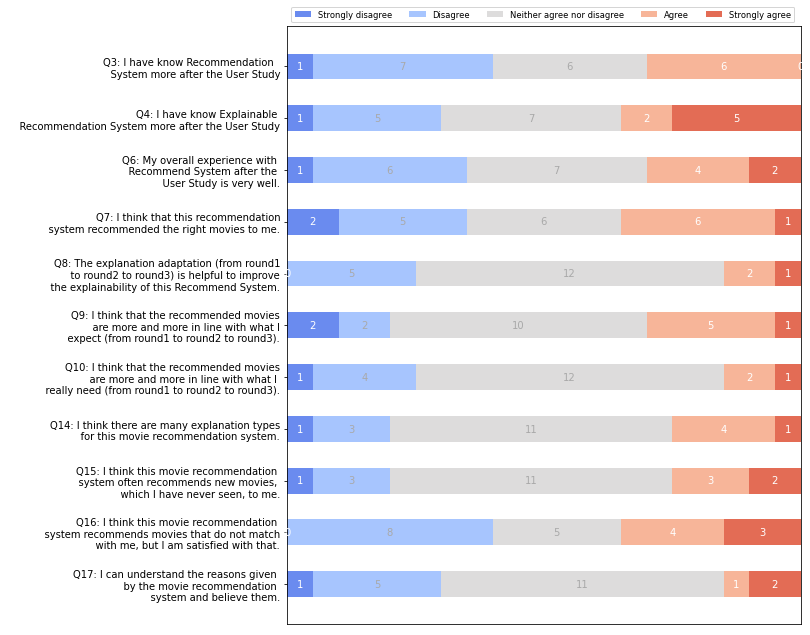
\includegraphics[width=1\textwidth]{feedback_question3}
\end{figure}

Figure \ref{figure:2} presents the results obtained from the preliminary analysis of points for 3 round recommendations from 20 users. We can see that the third round reported more high-points than the other two rounds.

\begin{figure}[h]
\caption{Feedback question about 3 round recommendations}
\label{figure:2}
\centering
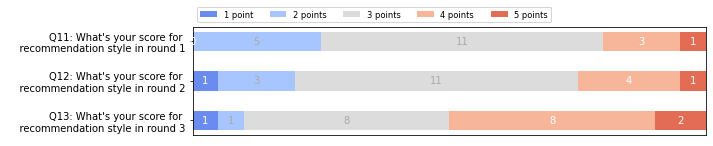
\includegraphics[width=1\textwidth]{feedback_question2}
\end{figure}



\subsection{User Study Metric}
Correspondingly, the division of questions for evaluating the recommendation system is shown in the table \ref{table:1}.

\begin{table}[h!]
\renewcommand\arraystretch{1.5}
\centering
\begin{tabular}{p{80pt}p{60pt}p{120pt}}\toprule
 \hline
 System Evaluation & Question & Result \\ [0.5ex] 
 \hline
  Satisfaction & Q6,Q8 & ...  \\
  Accuracy  & Q9,Q10 & ... \\ 
  Diversity & Q14 & ... \\
  Novelty & Q15 & ... \\
  Surprise & Q16 & ... \\
  Trust & Q17 & ... \\
  [1ex] 
 \hline
\end{tabular}
\caption{Questions for system evaluation}
\label{table:1}
\end{table}

\paragraph{Confidence}
\paragraph{Transparency}
\paragraph{Satisfaction}
\paragraph{Persuasiveness}
	
\subsection{Result analysis}

\cleardoublepage